\chapter{Исследовательская часть}

\section{Технические характеристики}

Технические характеристики устройства, на котором выполнялись замеры по времени выполнения реализаций, представлены далее.

\begin{itemize}
	\item Процессор: Intel(R) Core(TM) i7-1165G7 CPU 2.80 ГГц.
	\item Количество ядер: 4 физических и 8 логических.
	\item Оперативная память: 15 Гбайт.
	\item Операционная система: Ubuntu 64-разрядная система версии 22.04.3.
\end{itemize}

При замерах времени выполнения реализаций ноутбук был включен в сеть электропитания и был нагружен только системными приложениями.

\clearpage

\section{Замеры времени выполнения реализаций однопоточной и многопоточной реализации}
% TODO: написать разницу между процессорным временем и реальным, обьяснить почему в этой лабе используем реальное, пиши в аналит
Для замеров времени использовалась функция получения значения системных часов $clock()$~\cite{c-lang-time}.
Функция применялась два раза --- в начале и в конце измерения времени, значения полученных временных меток вычитались друг из друга для получения времени выполнения программы.

Исходный файл заполнялся случайными буквами латинского алфавита, цифрами и пробелами.
Размер исходного файла --- 500 МБ.

Средний размер строки --- 5500 символов.

Замеры проводились по 1000 раз для количества потоков от 1 до 25 и для однопоточной программы. Значение количества потоков 0 соответствует однопоточной программе, а значения n больше 0 — программе, создающей n дополнительных потоков, обработывающих строки.

В таблице \ref{tbl:time_tf} представлены замеры времени выполнения программы в зависимости от количества потоков.
\begin{table}[ht]
	\small
	\begin{center}
		\caption{Результаты нагрузочного тестирования (в мс).}
		\label{tbl:time_tf}
		\begin{tabular}{|r|r|}
			\hline
			\bfseries Кол-во потоков & \bfseries Время, мс
			\csvreader{csv/results.csv}{}
			{\\\hline \csvcoli & \csvcolii} \\
			\hline
		\end{tabular}
	\end{center}
\end{table}

\clearpage

На рисунке \ref{plt:res_graph} представлены результаты замеров.

\begin{figure}[h]
	\centering
	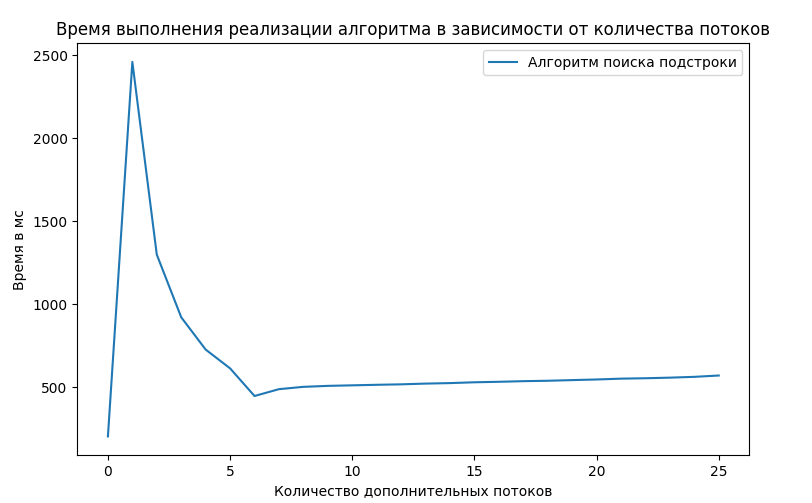
\includegraphics[height=0.35\textheight]{img/graph.png}
	\caption{Результаты замеров времени работы реализации алгоритма в зависимости от количества дополнительных потоков}
	\label{plt:res_graph}
\end{figure}

Из полученных результатов можно сделать вывод, что однопоточный процесс работает быстрее процесса, создающего вспомогательный поток для поиска подстрок в файле.
Это связано с дополнительными временными затратами на создание потока и передачи ему необходимых аргументов.
Наилучший результат по времени для многопоточной реализации для показал процесс с 6 дополнительными потоками, обрабатывающими строки. Так как используются еще 2 дополнительных потока - читатель и писатель, итоговое количество дополнительных потоков равно 8, что соответствует количеству логических ядер устройства.
Для числа потоков, большего данной величины, затраты на содержание потоков превышают преимущество от использования многопоточности, и функция времени от количества потоков начинает расти.

Временные затраты однопоточной реализации были меньше многопоточной при всех рассматриваемых количествах потоков, что объясняется затратами времени на передачу данных между потоками.

\section{Вывод}
В результате замеров было выявлено, что увеличение количества потоков может увеличить производительность для многопоточной реализации, однако затраты времени на поддержку множества потоков и передачу данных между ними приводит к увеличению временных затрат по сравнению с однопоточной реализацией.

Выборка из результатов замеров времени (для 5632 документов):
\begin{itemize}
	\item однопоточный процесс --- 203 мс;
	\item один дополнительный поток, выполняющий все вычисления --- 2459 мкс;
	\item 6 потоков (лучший результат) — 447 мкс, что в 5.5 раз быстрее выполнения процесса с одним потоком;
	\item 25 потока (худший результат) — 570 мкс, что в 4.3 раза быстрее выполнения процесса с одним потоком.
\end{itemize}

Таким образом, однопоточная реализация затрачивает меньше времени при любом количества дополнительных потоков многопоточной программы.
Добавление дополнительных потоков может как ускорить выполнение многопоточной программы, так и замедлить.
Рекомендуется использовать на данной архитектуре ЭВМ число дополнительных потоков, равное числу логических ядер устройства.
